% This is main.tex, a sample paper demonstrating the use of the
% LLNCS macro package for Springer Computer Science proceedings;
% Version 2.20 of 2017/10/04
% 
\documentclass[runningheads]{llncs}
\usepackage[a4paper,left=3cm,right=3cm,top=4cm,bottom=4cm,bindingoffset=5mm]{geometry}
%
% ---- Packages ----
%
\usepackage{graphicx} % enhanced support for graphics
\usepackage{url} % add macros for handling URLs in text
\usepackage[nohyperlinks,nolist]{acronym} % abbreviation utilities
\usepackage{listings}
% TODO: add more packages below if necessary
%
% ---- Acronyms ----
%
\begin{acronym}
\acro{rq}[RQ]{Research Question}
\end{acronym}
%
% ---- Begin Document ----
%
\begin{document}
\title{NLP Selection of Tests - ...}
\author{Marius Bosler}
\institute{Seminar: Software Quality\\
Advisor: Roland Würsching\\
Technical University of Munich\\
\email{marius.bosler@tum.de}}
%
\maketitle % typeset the header of the contribution
%
% ---- Abstract ----
%
\begin{abstract}
Even though there have been many advancements in recent years, a significant amount of testing still needs to be conducted manually. This means that with each software release requiring numerous manual tests, a considerable amount of time is spent executing these tests. Meanwhile, many of these tests tend to overlap in bug detection, which could be avoided if a method were found to execute only the necessary number of tests, as multiple tests may detect the same bug. One way to achieve this is by clustering them through an analysis of the language used in their description. Then, by carefully selecting only a subset of all tests based on said clustering, a lot of time can be saved, especially if the selected tests cover a significant portion of the detected bugs.

\keywords{Test Selection, Natural Language Processing, Clustering}
\end{abstract}
%
% ---- Text Parts ----
%
\section{Introduction}

In the evolution of software testing, a key goal has always been to make testing faster and more reliable. And even though much can be automated nowadays, it is oftentimes still preferable to use manual instead of automated tests, as they are comparatively easy to create and change. One problem with manual testing, however, is that it usually takes a lot of time and human effort to run the tests. Additionally, tests might often have an overlap with each other, because, among other things, for larger projects many test case maintainers do not know every other test case by heart and therefore might introduce redundancy which is of course especially to be avoided in the case of manual tests that take a long time to execute.

Our approach aims to mitigate this redundancy by examining the relationship between test cases. For instance, if two tests A and B have similar textual descriptions, it might be that they cover similar functionalities and therefore potentially detect the same bugs, so in this case, we might want to only execute Test A and thereby reduce our test execution time significantly, even though we still find both bugs. 

A lot of ways to find similar tests like this have been proposed, mostly by analyzing the textual descriptions of these tests, like in the study by Viggiato et al. \cite{Viggiato}. In that study, \ac{NLP} was used on the test steps to find similar test cases, then clustering said test cases to find similar ones.

Recognizing that many tests redundantly identify the same bugs, this study aims to build on the mentioned approach in that study, to later select only a subset of said tests based on their similarity and thereby hopefully reduce the test cases that need to be executed drastically, while still covering a significant portion of recognized bugs.

In our case, we will use a dataset from XWiki, an open-source wiki platform with 1,600 manual tests. If one of these tests fails during execution, the testers append a Bug Ticket to the test. We will use these Bug tickets to discover and evaluate said redundancies.

The entire approach was implemented in Python because of its ease of use and because it has one of the best library support in the fields we look at, especially in the field of \ac{NLP}.
\section{Related Work}

To solve the problem of test selection, a lot of approaches have been proposed. Of particular interest to us is test case selection using \ac{NLP}. In that field, the work by Sutar et al. \cite{Sutar} stands out prominently. Sutar et al. proposed a method to select regression test cases based on their relevance to defects using \ac{NLP}. In their approach, they focus on regression testing, analyzing both software requirements and test case descriptions using \ac{NLP}. By calculating the similarity between these, they prioritize those test cases that are most likely to be impacted by changes to the code. However, in this paper, we want to focus not only on regression test case selection but on general test case selection.

Another influential approach for this paper is the one proposed by Li et al. \cite{Li}. The researchers use \ac{NLP} to group semantically similar test steps across different test cases and then cluster these steps to reveal which ones likely perform the same or similar actions. This allows for the avoidance of duplicate or overlapping API methods when the tests are automated. Although the goal of that paper is not the same as ours, they used a similar approach that this paper will explore.

The fundamental approach to finding test similarity in this paper is mostly based on the paper by Viggiato et al. \cite{Viggiato}. The researchers use \ac{NLP} to identify similar test steps within test cases. Text embedding models then convert the text of test steps into numerical representations. These textual similarities are used to determine how closely related the tests with these embedded steps are, followed by clustering to group similar test cases. This step-level analysis aims to reduce redundancy within the overall test suite.

This paper aims to combine the mentioned \ac{NLP} approaches and introduce real-life bug data by XWiki to improve test case selection compared to random selection. We will use the method by Viggiato et al. to cluster embeddings of test steps, and then cluster test cases based on these clusterings. Finally, we will select test cases with that second clustering, validating the approach for finding test case similarity and demonstrating a potential use case of the proposed method.
\section{Methodology}
\subsection{Data Collection and Description}
We used data from XWiki, an open-source wiki platform. From their website, we scraped a dataset of 1,600 manual test cases and 52,860 test executions. Each test case is structured with a description, title, steps to reproduce, and expected results. For instance, a typical test case might look like this:

\begin{Verbatim}[fontsize=\small]
    "https://test.xwiki.org/xwiki/bin/view/File%20Manager%20Tests/Delete%20a%20file": {
        "title": "Delete a file",
        "steps_to_reproduce": [
            "Click on File Manager from Applications Panel",
            "Click on All Files",
            "Select a file",
            "Click on Delete",
            "Click on OK"
        ],
        "expected_result": [
            "The file is deleted."
        ]
    }
\end{Verbatim}

The dataset chosen for this study is especially fitting for us because it contains detailed textual descriptions in the form of test steps. These descriptions can help determine the similarity between tests, which we can use to cluster them together.

\subsection{\ac{NLP} Techniques and Test Selection Process}

To find similar test cases, we use a mix of text embedding and clustering. The approach to finding similar test cases is based on the approach by Viggiato et al. \cite{Viggiato}.

First, we converted all words to lowercase and used word stemming, with the python library \emph{nltk}.
For example, this converts the sentence \emph{Click on File Manager from Applications Panel} to important word stems: \emph{click file manag applic panel}. \\
This is done to make text analysis more efficient, especially if we only want to extract the meaning and similarity of test steps.

We then converted the resulting strings to their embeddings with the Python library \emph{SentenceTransformer} and the model \emph{all-mpnet-base-v2}. Embeddings can be thought of as representations of textual information in a numerical format. This is important because they enable us to efficiently compare similarities between different elements mathematically.
Every sentence is now represented as a vector of numbers with a length of 768:

\begin{Verbatim}
[-8.30066670e-03, -4.04462852e-02, -2.05343179e-02,  3.46409194e-02,
\end{Verbatim}
\vdots
\begin{Verbatim}
1.46980640e-02,  3.09091341e-02,  3.18837278e-02,  3.14172916e-02]
\end{Verbatim}

To then find similarities between test cases, we needed to find a way to find out which tests have similar test steps. This is done in the following way:
First, we are clustering the embeddings of all test steps, so every test case has several clusters whose test steps are in. As a simplified example, we might sort them into 10 clusters, then our example test case steps might be in the clusters with ids \emph{4, 2, 2, 6, 7} (the results are better if we use much more than 10 clusters).
For the actual clustering of test cases, we've employed three distinct algorithms: KMeans, DBScan, and Optics. After some evaluation, it became clear that KMeans was the most fitting choice for our specific needs, as we later want to choose the \emph{n} dissimilar test cases and KMeans lets us define how many test clusters we want.
Then we need to find similarities between actual test cases:
For every test case, we create an empty null vector with the length of the number of different clusters. Then we fill it at the positions of said cluster IDs with how many each cluster appears:

\begin{Verbatim}
    [0, 0, 2, 0, 1, 0, 1, 1, 0, 0]
\end{Verbatim}



\begin{figure}[H]
    
\noindent\makebox[\textwidth][l]{%
    \hspace{\dimexpr\oddsidemargin-3cm}%
        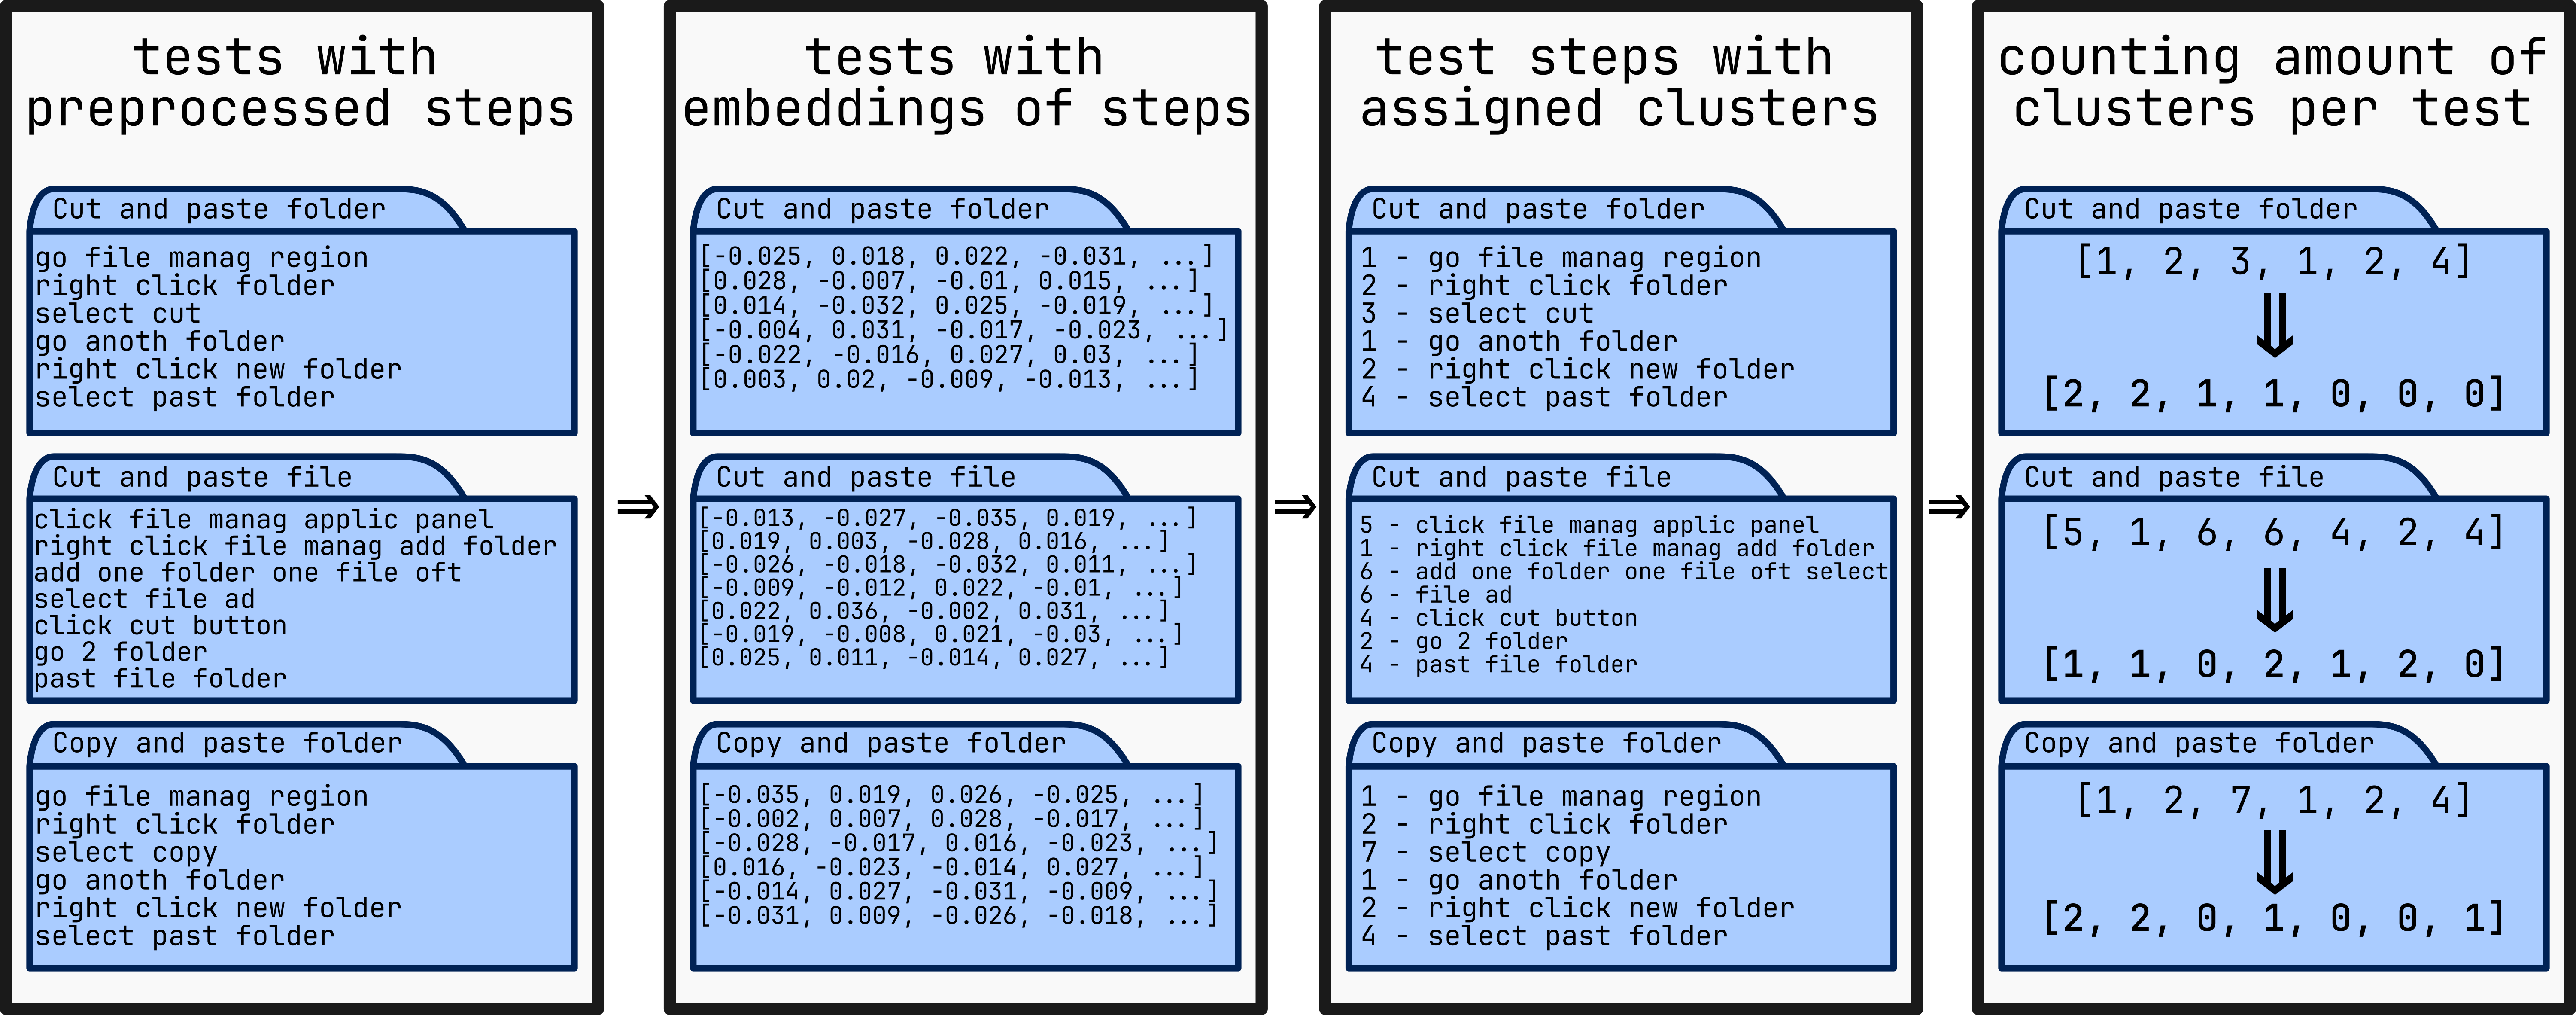
\includegraphics[width=0.9\paperwidth]{figures/getting_representation_for_tests.png}%
}
\caption{Getting a vector representation for each test}

\end{figure}


These Vectors now represent our tests in a mathematical way, which, as mentioned earlier, we want to compare the tests with other tests.
To achieve this, we cluster again after these vectors and as we want to select \emph{n} dissimilar test cases, we cluster with KMeans to cluster the tests into \emph{n} clusters.

After that, we have \emph{n} clusters of test cases from which we then randomly select one test each. This will be our test selection.

\section{Evaluation}
\subsection{Research Questions}
To test our approach, we want to use our dataset of XWiki to answer the following  \acp{rq}:
\begin{itemize}
    \item \ac{rq}1: Does clustering test cases by test steps cluster similar tests?
    Each test consists of a number of test steps to execute when executing the tests. It is not given that clustering these test steps actually gives us a clustering that clusters similar test cases together.
    \item \ac{rq}2: How much time/many tests can be saved by selecting tests based on clustering test cases by test steps?
    The goal of this paper is to demonstrate wether clustering tests in said method can produce helpful results. But is there actually a substantial amount of time/tests that can be saved when only selecting a portion of all tests?
    \item \ac{rq}3: Does the proposed method pose a threat to fault coverage if only a subset of tests are executed?
    \item \ac{rq}4: What is an appropriate amount of tests to be executed without threatening the fault coverage too much?
    \\\\\indent{alternatively (shorter):}
    \item \ac{rq}1: Does clustering test cases by steps effectively group similar tests and reduce test count or time?
    \item \ac{rq}2:Does clustering test cases by steps effectively reduce test count or time?
    \item \ac{rq}3: What balance ensures optimal fault coverage with minimum tests after clustering?
\end{itemize}
\section{Discussion}

This section shall discuss the results and the research questions to analyze the effectiveness of our approach.

\ac{rq}1: \emph{How many bug tickets are found when selecting only a subset of tests using NLP-Clustering by Test Specification}


With the \ac*{NLP}-based approach we cover a much bigger portion of bugs than the amount of tests that were executed. With $\frac{1}{2}$ of tests selected we find nearly $\frac{3}{4}$ of bug tickets. This is a relatively satisfactory result, especially considering so little information was used to compare the tests. 
At the same time, we are sadly missing out on a lot of bugs we used to discover when selecting 100\% of tests.
However, a large project such as the XWiki project or other even larger ones might often have problems finding enough people to execute the tests on every new version, especially when the number of manual tests keeps rising. On smaller versions, it might therefore be preferable to only choose as many test cases as can be executed in a realistic amount of time until release.
So, if a project has a problem with manual testers, this approach achieves a reasonable tradeoff between time spent and bugs found.

\ac{rq}2: \emph{How does the performance of NLP-based test selection compare with simpler, more naive methods of test selection in terms of bug detection?}

As for the first naive approach, the number of bug tickets we cover when selecting completely random is percentage-wise higher than the amount of tests we select. This occurs because many test cases are associated with multiple bug tickets. As a result, a test case might cover a higher percentage of bug tickets than its proportion within the test suite would suggest. But still, the number is drastically less than the proposed \ac{NLP}-based approach. With 50\% of tests selected, we only find close to 55\% of bug tickets, so nearly 20\% less, showing a significantly improved performance for the \ac{NLP}-based approach.

The next naive approach was to select based on categories. Selecting 30\% of test cases from separate categories first showed a bug detection quota of 38.53\%. This result was somewhat surprising because one might expect a significantly better result than just choosing tests randomly. After all, the categories show an intrinsic test similarity based on human judgment. That this did not significantly improve bug coverage showed us how difficult it might be to improve upon random selection.

All in all, the proposed approach to selection gave us a significantly better selection compared to more naive approaches. Given the fact that executing the algorithms on a system with an intel i7-12850HX with 16 cores only takes about 3.5 minutes, which is barely noticeable when comparing that to the time we might use for executing hundreds of tests, we can recognize a drastic reduction in time spent executing manual tests, which could also lead to a faster release of new versions.


\section{Threats to Validity}

\subsection*{External:} 
The dataset of XWiki might not represent all manual test suites equally. It is possible that the suite was a lucky choice for our approach and other datasets might not have the same level of improvements over random selection. If the XWiki dataset has bug distributions significantly different from what is commonly seen in software projects (e.g., very few bugs concentrated in a small portion of the system), it might limit the generalizability of the findings.
Also, if the quality of test case descriptions varies significantly (level of detail, clarity etc.), it could weaken the quality of the NLP analysis and clustering.


\subsection*{Internal:} 
There might be some bugs that are more important or take more time than others. If the \ac{NLP}-based approach only selects dissimilar tests, we might have a bias on not executing a set of more important test cases if they are too similar to each other and thereby might not find a set of more important bugs.
While textual similarity of test case steps leads to an improvement of bug coverage in our case, it is not guaranteed that it actually effectively identifies test similarity all the time. Not every relation between tests might be covered by textual similarity and there might even be datasets where the textual similarity does not at all correlate with similar code that is tested in the background. This could lead to drastically worse results on other datasets.

\subsection*{Mitigation}
To avoid these threats one might want to introduce bigger datasets and also look at the severity of bugs. On top of that, manually identifying similar tests might give an idea of how good \ac{NLP}-based similarity works to find similar tests compared to other approaches and might display inadequacies of this approach.
Also, including other parts of the test case descriptions and a different way to cluster the embeddings could improve bug coverage even more and make the \ac{NLP}-based approach work on more datasets that might not work with our exact approach.

\section{Conclusion}
\label{sec:conclusion}

You can also reference other parts of the document, e.g., sections or subsections.
In Section~\ref{sec:intro} we briefly introduced something, whereas in Subsection~\ref{sec:intro:sub:motivation}, we motivated something else.

Make sure to capitalize chapters, sections or subsections when referencing them.
%
% ---- Bibliography ----
%
\bibliographystyle{splncs04}
\bibliography{library.bib}
%
\end{document}
